\begin{figure*}
    \centering
    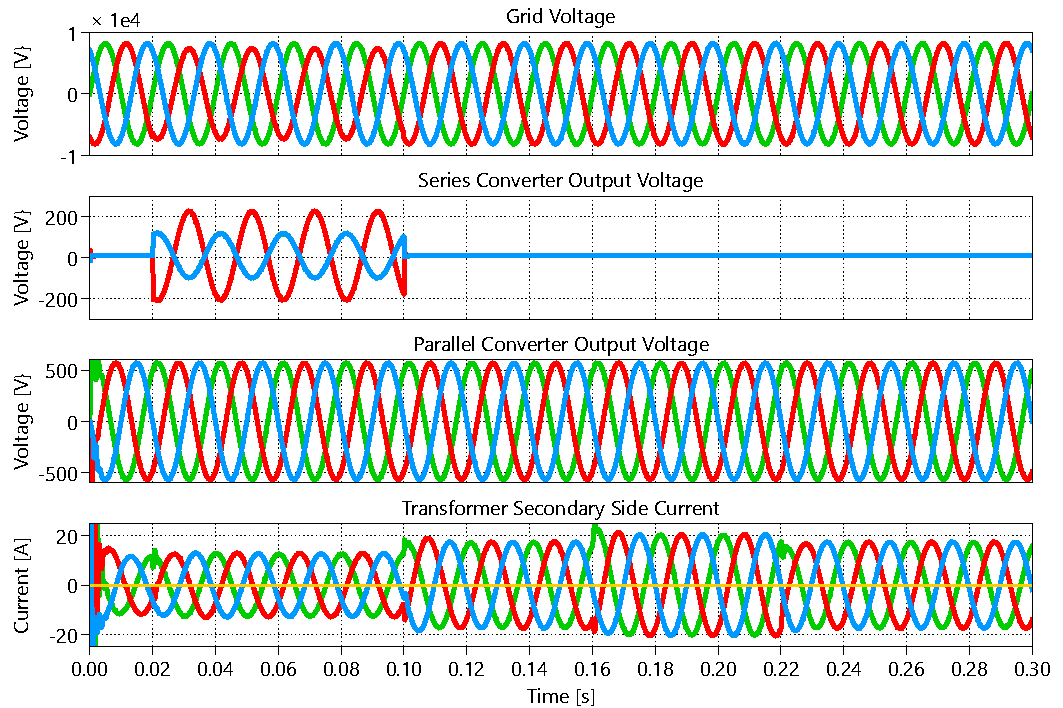
\includegraphics[width=\textwidth]{Images/Sim1.pdf}
    \caption{Simulation results for the proposed control strategy under grid and load disturbances.}
    \label{fig:sim1}
\end{figure*}

\begin{figure*}
    \centering
    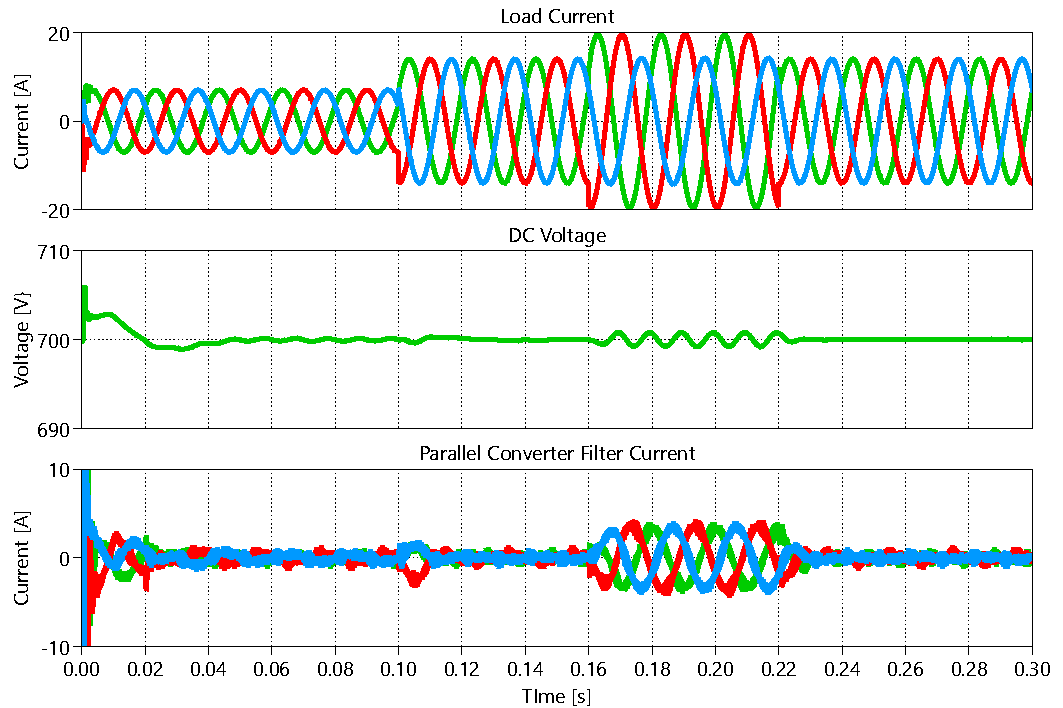
\includegraphics[width=\textwidth]{Images/Sim2.pdf}
    \caption{Simulation results for the proposed control strategy under grid and load disturbances.}
    \label{fig:sim2}
\end{figure*}

\begin{figure*}
    \centering
    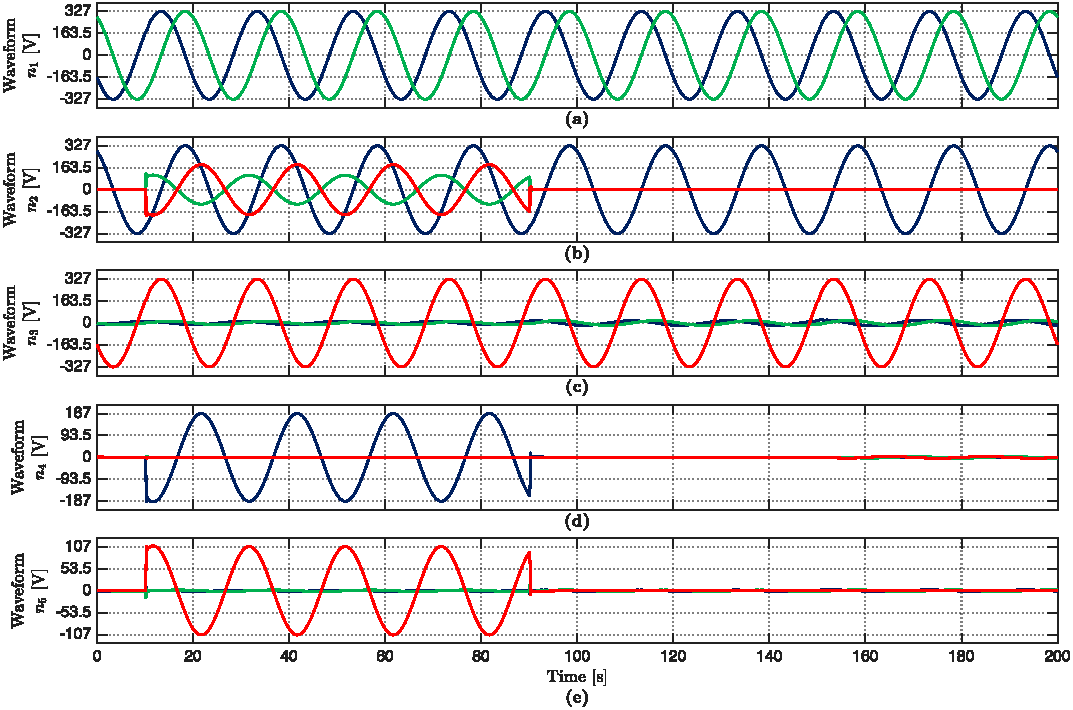
\includegraphics[width=\textwidth]{Images/Fig3_ex.pdf}
    \caption{Simulation results for the proposed control strategy under grid and load disturbances.}
    \label{fig:sim3}
\end{figure*}

In this section, the simulation results of the proposed control strategy are presented. The simulations are performed using MATLAB/Simulink, and the system parameters are listed in Table \ref{tab:params}. The proposed control strategy is tested under various grid and load disturbances, including grid voltage unbalanced swell, load impact, and unbalanced load.

\begin{table}[h!]
    \centering
    \caption{System Parameters}
    \begin{tabular}{|c|c|c|}
        \hline
        Parameter & Variable & Value \\
        \hline
        \hline
        Grid Voltage & $V_{g}$ & 10 kV \\
        Grid Frequency & $f_e$ & 50 Hz \\
        Transformers Power Rating & $S$ & 1 kVA \\
        DC Link Voltage & $V_{DC}$ & 400 V \\
        Series Converter Filter Inductance & $L_{fs}$ & 2 mH \\
        Series Converter Filter Capacitance & $C_{fs}$ & 20 µF \\
        Parallel Converter Filter Inductance & $L_{fp}$ & 2 mH \\
        Parallel Converter Filter Capacitance & $C_{fp}$ & 20 µF \\
        Transformer Dispersion Inductance & $L_Y$ & 0.1 mH \\
        Transformer Series Resistance & $R_Y$ & $50\ \Omega$\\
        Coupling Transformer Turns Ratio & $N_{ct}$ & $2.5$ \\
        Distribution Transformer Turns Ratio & $N_{DT}$ & $a$ \\
        Converters Switching Frequency & $f_{\text{sw}}$ & 20 kHz \\
        Control Sampling Time & $T_s$ & 5 µs \\
        \hline
    \end{tabular}
    \label{tab:params}
\end{table}


\subsection{Grid Voltage Unbalanced Swell Compensation}

The simulation results for the proposed control strategy under grid voltage unbalanced swell are shown in Fig. \ref{fig:sim1}. The grid voltage swell occurs at $t=0.02\ s$ and lasts for $0.08\ s$. The proposed control strategy effectively compensates for the voltage swell, maintaining a balanced load current. 
%\subsection{Grid Voltage Harmonics Compensation}

\subsection{Load Impact and Unbalanced Load Compensation}

In the other hand, a load unbalance is applied at $t=0.1\ s$ and lasts for $0.06\ s$. Then, an unbalanced load is applied at $t=0.16\ s$ and lasts for $0.06\ s$. The proposed control strategy effectively compensates for the load unbalance, meaning that the parallel inverter injects the necessary current to maintain a balanced load current, as shown in Fig. \ref{fig:sim2}.

%\subsection{Non-linear Load Compensation}

%\subsection{Load Harmonics Compensation}